\section{Introduction}

The arm966e\_s is a system level simulator of the ARM966E\_S processor. This simulator is a very simple simulator with just a memory connected to it. It is able to run any firmware loaded into the ram of the simulator, programs can use the full instruction set of those processors, including the Thumb instruction set. The simulator uses an elf binary loader to load into memory the firmware to simulate. Take into account that programs for those simulators require to be correctly mapped into the memory, refer to the processors manuals for more information. Software running on the simulated hardware can be debugged by connecting a GDB client to the simulator through the GDB serial remote protocol. The GDB client can be either the standard text based client (i.e. command gdb), a graphical front-end to GDB (e.g. ddd), or even Eclipse CDT. Additionally an inline debugger is also available.

The arm966e\_s does implement the CP15 coprocessor as described in the processor manual, and includes the integrated scratchpad memories (called TCM, tightly coupled memory). 

\begin{figure}[!h]
	\begin{center}
		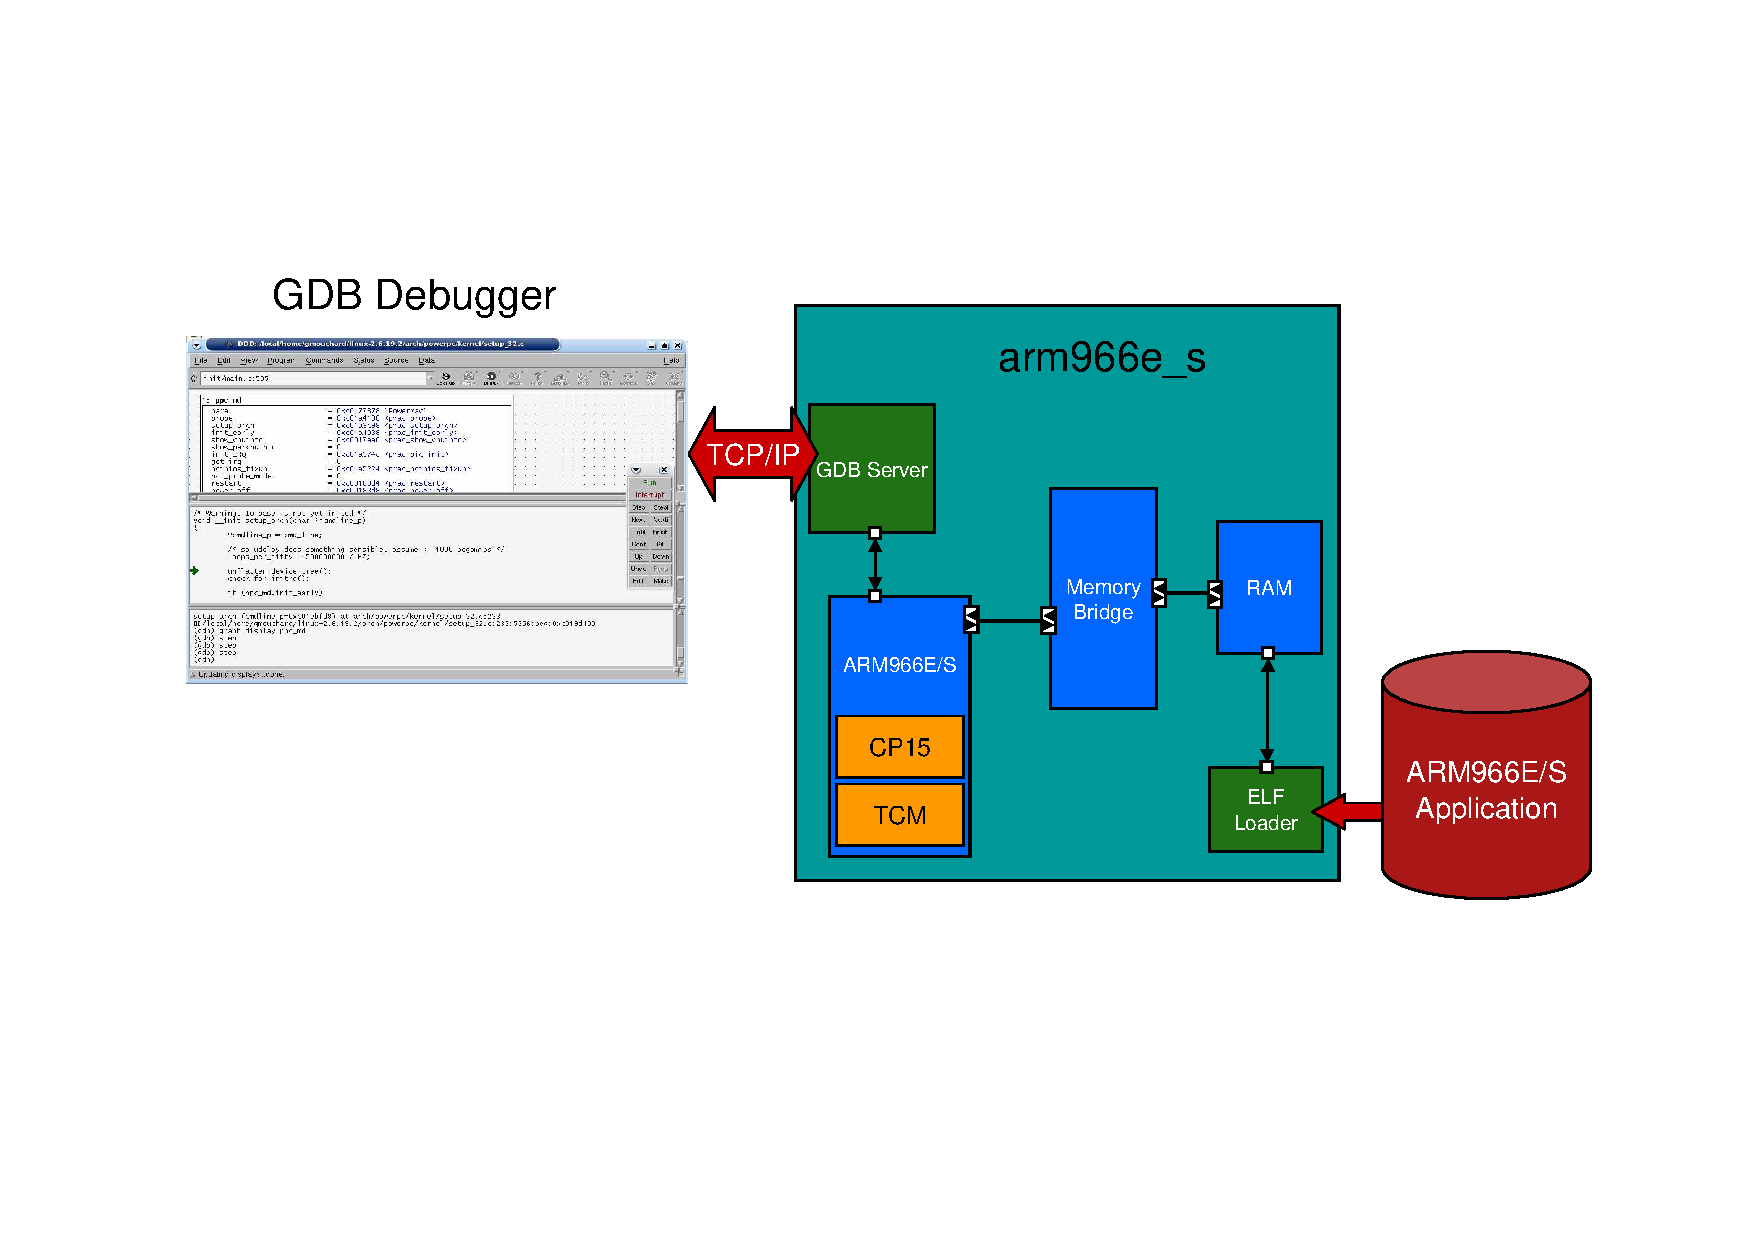
\includegraphics[width=\textwidth]{arm966e_s/fig_arm966e_s.pdf}
	\end{center}
	\caption{arm966e\_s simplified schematic.}
	\label{fig:arm966e_s}
\end{figure}

Two different versions of the simulator are available:
\begin{itemize}
	\item arm966e\_s: the ARM966E\_S simulator
    \item arm966e\_s-debug: the ARM966E\_S simulator with debug information to see (traces) what is happening inside the simulator (note: it is slow)
\end{itemize}

\section{Simulated configuration}

The simulator is composed of the following modules:
\begin{itemize}\addtolength{\itemsep}{-0.40\baselineskip}
\item ARM CPU configured as an ARM966E\_S
\item Simple bus to memory bridge
\item memory
\end{itemize}

The simulator uses the following services:
\begin{itemize}\addtolength{\itemsep}{-0.40\baselineskip}
\item ELF loader
\item GDB Server
\item Inline debugger
\item SystemC Time
\item Host Time
\end{itemize}

\section{Using the simulator}

Usage: \texttt{arm966e\_s [<options>] <program> [program arguments]}

     'program' is statically linked ELF32 ARM Linux program

Options:
\begin{itemize}
\item Displaying the integrated help

\texttt{--help}
\texttt{-h}

\item Getting the simulation default configuration variables into a XML file\\
\texttt{--get-variables <xml file>}\\
\texttt{-v <xml file>}

\item Configuring the simulator with the given XML configuration file\\
\texttt{--config <xml file>}\\
\texttt{-c <xml file>}

\item Getting the simulator default configuration XML file\\
\texttt{--get-config <xml file>}\\
\texttt{-g <xml file>}\\

Note: you can use it as a template to create your own XML configuration file.

\item Activating the logger\\
\texttt{--logger}\\
\texttt{-l}

\item Defining the XML processor description file for GDB\\
\texttt{--xml-gdb <file>}\\
\texttt{-x <file>}

\item Activating the GDB server\\
\texttt{--gdb-server <port\_number>}\\
\texttt{-d <port\_number>}\\
           
Note: GDB server will use the given port\\

\item Activating the inline debugger\\
\texttt{--inline-debugger}\\
\texttt{-i}

\item Activating message spies\\
\texttt{--message-spy}\\
\texttt{-m}
\end{itemize}

The arm966e\_s simulator provides few options, but you can highly configure them using XML configuration file. To have a canvas of the XML configuration file simply run the simulator with the following option:
\begin{verbatim}
-g <xml file>
\end{verbatim}

This will generate an XML file describing the default configuration of the simulator. The following code shows you part of the initial xml configuration of the arm966e\_s:
\begin{verbatim}
<?xml version="1.0" encoding="UTF-8"?>
<VARIABLES>
  <variable>
    <type>parameter</type>
    <name>bridge.fsb-cycle-time</name>
    <data_type>unsigned long long</data_type>
    <default_value>0x0</default_value>
    <value>0x0</value>
    <description></description>
  </variable>
  <variable>
    <type>parameter</type>
    <name>bridge.mem-cycle-time</name>
    <data_type>unsigned long long</data_type>
    <default_value>0x0</default_value>
    <value>0x0</value>
    <description></description>
  </variable>
...
</VARIABLES>
\end{verbatim}

Modify the value field of the configuration parameters as you wish to set up your personal configuration, and use the -c option on the simulator to launch the simulation with your modified configuration file.
